\section{Satisfiability}


\begin{frame}[noframenumbering]
	
\vfill
\centering

\vspace{-.5cm}\textbf{\Large Satisfiability in Quantum Circuit Compilation}\vspace{-.5cm}

\vfill

\centering
\alert{(A very incomplete overview)}

\end{frame}



\begin{refframe}{SAT-based Quantum Circuit Simulation}


\vspace{-6em}

\cols{
\col{6cm}{}
\col{4cm}{
\begin{itemize}
\item[\color{green}\cmark] Efficient SAT encoding
\item[\color{red}\xmark] Non-universal
\end{itemize}
}}
\pause


\begin{block}{Berent et al. --- Towards a SAT Encoding for .. \cite{berent2022towards}}
\begin{itemize}
%\item Exponential-length encoding of universal circuits (requiring a simulator)
%\pause
\item Stabilizer circuit simulation  			\hfill (non-universal)
\item Stabilizer circuit equivalence checking	\hfill (non-universal)
\end{itemize}
\end{block}


\onslide<2->{

\tikzset{venn circle/.style={circle,minimum width=2cm,fill=####1,opacity=0.4}}
\begin{tikzpicture}[
e/.style = {ellipse, fill=####1, draw=none,
            minimum height=.7cm, minimum width=.9cm, inner sep=0pt},
e/.default=black
]
\footnotesize


%\draw[help lines] (0,0) grid (4,3);


%  \node [e = yellow!0!red!80!white,text width=2.8cm,align=center, minimum width=.8cm,  minimum height=3.6cm,text opacity=1,label={[anchor=north, inner sep=3pt,yshift=-.25cm]north:Precise\QMA = \PSPACE}] (PSPACE) at (.8,0.5) {};
%	\node[right = of PSPACE.north east] (ECEQ) {\color{red} \textbf{Exact} quantum circuit non-equivalence};
%	\draw[-Circle,shorten >= -.2cm] (ECEQ) -- (PSPACE.north east);
%
%
%
%  \node [e = yellow!30!red!80!white,text width=2.3cm,align=center, minimum width=.8cm,  minimum height=2.8cm,text opacity=1,label={[anchor=north, inner sep=3pt,yshift=-.2cm]north:Precise\BQP = \PP}] (PP) at (.8,0.3) {};
%	\node[right = of PP.north east] (EQCSIM) {\color{OliveGreen} \textbf{Exact} quantum circuit simulation};
%	\draw[-Circle,shorten >= -.2cm] (EQCSIM) -- (PP.north east);



  \node [e = yellow!40!red!50!white,text width=2cm,align=center, minimum width=.8cm,  minimum height=2cm,text opacity=1,label={[anchor=north, inner sep=3pt]north:\QMA}] (QMA) at (.75,0.1) {};
	\node[right = of QMA.north east] (CEQ) {\color{red} Quantum circuit non-equivalence};
	\draw[-Circle,shorten >= -.2cm] (CEQ) -- (QMA.north east);


	\node [venn circle = yellow!80!red,text width=1cm,align=center, minimum width=.8cm,opacity=.5,text opacity=1,label={[anchor=west, inner sep=3pt]north west:\NP}] (NP) at (0,0) {};
	\node[left = of NP] (SAT) {\color{red}  Circuit non-equivalence};
	\draw[-Circle,shorten >= -.18cm] (SAT) -- (NP);
  
  
	\node[e = blue!80!white, opacity=0.5, minimum height=1cm] (BQP) at (1,0) {~~~~~~~~~~~~~~~\BQP};
  \node[below right = of BQP,text width=3cm] (QCS) {\color{OliveGreen} Quantum circuit simulation};
  \draw[-Circle,shorten >= -.18cm] (QCS) -- (BQP);
	
	
	\node [e = blue!60!white, opacity=.7] at (.5,0) {~~~~~~\BPP};


  \node [venn circle = blue!80,text width=.3cm,align=center, minimum width=.3cm,opacity=.5,text opacity=1] (P) at (.2,0) {{~~\P}};  
  \node[below left = of P] (CVP) {\color{OliveGreen} Circuit evaluation (simulation)};
  \draw[-Circle,shorten >= -.18cm] (CVP) -- (P);



	\node<3->[below = of P.south,text width=4cm,xshift=.5cm,yshift=-.2cm] (Clifford) {\centering \color{blue} Stabilizer circuit simulation \cite{aaronson2008improved} /\\ Stabilizer circuit non-equivalence \cite{ours}};
	\draw<3->[-Circle,shorten >= -.2cm] (Clifford) -- (P.south);

\end{tikzpicture}	

}


%\pause[5]
%\centering
%\alert{Hardness gap: adding e.g. a $T$ gate brings us from \P{} up to \PSPACE/\PP }

\end{refframe}




\begin{refframe}{SMT-based Quantum Circuit Simulation}

\vspace{-3em}

\cols{
\col{6cm}{}
\col{4cm}{
\begin{itemize}
\item[\color{red}\xmark] Intractable SMT theory
\item[\color{green}\cmark] Universal
\end{itemize}
}}
\pause


\begin{block}{symQV: Automated Symbolic Verification of ... \cite{bauermarquart2023symqv}}
\begin{itemize}
\item<+-> Efficient SMT-encoding of \alert{universal} quantum circuits
\item<3-> Uses \alert{undecidable} theory: NLA with trigonometric expressions
\item<3-> Limited scaling
\end{itemize}
\end{block}

\onslide<2->{
\centering
\scalebox{1.3}{
$
	\vec v   =
	\def\arraystretch{1.3}
%    \left.
    \begin{bmatrix*}[c]
     \sqrt i \\0 \\ 0\\ 0 \\ \vdots \\ 0 \\ 0\\ 0  \\
    \end{bmatrix*}
%    \right\}\text{ $2^n$ complex \alert{probability amplitudes}}
$
}
}
	
\end{refframe}




\begin{refframe}{\#SAT-based Quantum Circuit Simulation}

\vspace{-3em}

\cols{
\col{6cm}{}
\col{4cm}{
\begin{itemize}
\item[\color{green}\cmark] Efficient \#SAT encoding
\item[\color{green}\cmark] Universal
\end{itemize}
}}
\pause


\begin{block}{Simulating Quantum Circuits by Weighted Model Counting (WMC)\cite{mei2024simulating}}
\begin{itemize}
\item<+-> Use density matrix instead of state vector
%\item<6-> Represent in Pauli basis, i.e., $\rho = \sum_j  \alpha_j P_j$  
%\item<7-> \alert{Obviates the need for complex weights $\alpha_j$}
\item<4-> \alert{Result: WMC encoding of length $\mathcal O(n +m)$ for $n$ qubits and $m$ gates}
\item<5-> Negative weights: \alert{constructive and destructive interference}
\end{itemize}
\end{block}

\onslide<2->{
\scalebox{1.}{
\hspace{-2.5em}
$
	\rho  = \vec v \cdot \vec v^{\dagger}   = \onslide<2->{
	\def\arraystretch{1.3}
    \begin{bmatrix*}[c]
     \tfrac{\sqrt i}{\sqrt 2} \\0 \\ 0\\ \vdots \\ 0 \\ \tfrac{1}{\sqrt 2}\\ 0  \\
    \end{bmatrix*}\cdot 
    \begin{bmatrix*}[c]
     \tfrac{\sqrt i}{\sqrt 2}^* & 0 & 0&  \dots & 0 & \tfrac{1}{\sqrt 2}^* &  0  
    \end{bmatrix*} =  \onslide<3->{ 
    \begin{bmatrix*}[c]
     \tfrac{1}{2} & 0 & 0&  \dots & 0 & \tfrac{\sqrt i}{2} &  0 \\ 
     0 & 0 & 0& \dots & 0 & 0 &  0 \\ 
     0 & 0 & 0& \dots & 0 & 0 &  0 \\ 
     0 & 0 & 0& \dots & 0 & 0 &  0 \\ 
     \vdots & \vdots & \vdots  & \dots & \vdots & \vdots &  \vdots \\ 
     0 & 0 & 0 & \dots & 0 & 0 &  0 \\ 
     0 & 0 & 0 & \dots & 0 & 0 &  0 \\ 
     \tfrac{\sqrt i^*}{2}  & 0 & 0 & \dots & 0 & \tfrac{1}{2} &  0 \\ 
     0 & 0 & 0 & \dots & 0 & 0 &  0 \\ 
    \end{bmatrix*} 
    }}
%    \right\}\text{ $2^n$ complex \alert{probability amplitudes}}
$
}
}


%for $P_j \in\set{I, X, Y, Z}$
\end{refframe}




\begin{refframe}{\#SAT-based Quantum Circuit Simulation}

Simulating Quantum Circuits by Weighted Model Counting (WMC) \cite{mei2024simulating}

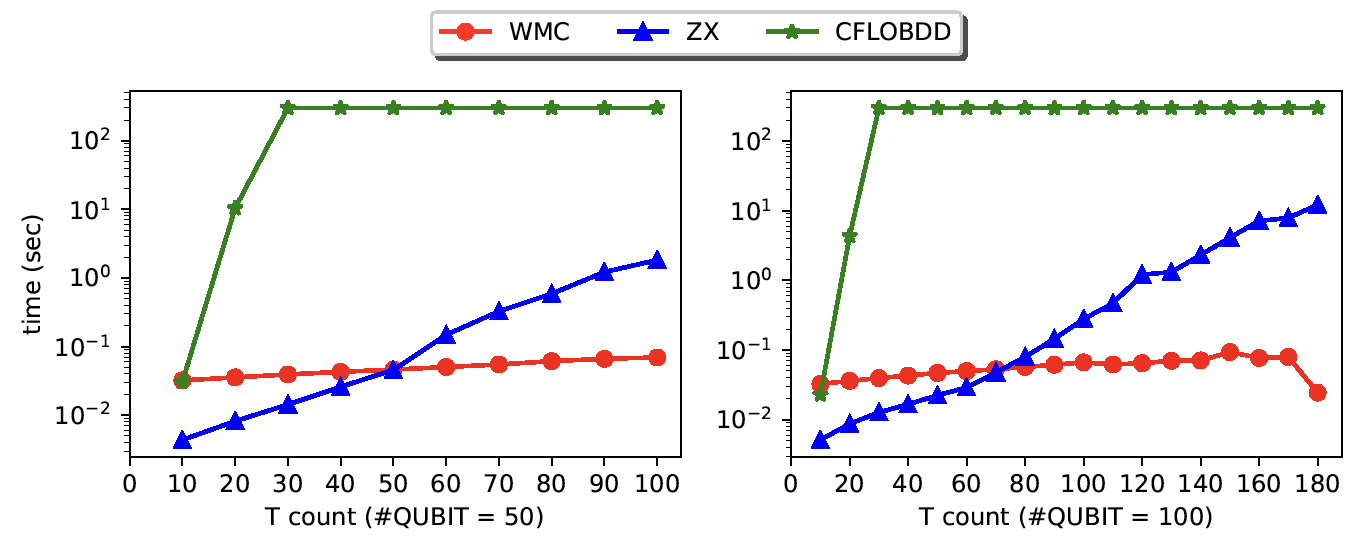
\includegraphics[height=4.5cm]{graphics/random-quokka}

	
\end{refframe}



%
\begin{refframe}{\#SAT-based Quantum Circuit Simulation}

\begin{block}{Equivalence Checking ... by Weighted Model Counting (WMC)\cite{mei2024eq}}
\begin{itemize}
\item<+-> Use the same $\mathcal O(n +m)$ WMC encoding
\item<+-> Combine with equivalence checking theorem from~\cite{ours} 
%\\\hfill (Pauli basis is generated by only $2n$ elements)
\end{itemize}
\end{block}


\begin{alertblock}<+->{Opportunities for both \#SAT-based approaches}
\begin{itemize}
\item<.-> Optimize (weighted) model counters for quantum problems (XOR constraints)
\item<+-> Support of negative weights in approximate counters and samplers
\item<+-> \alert{Synthesis for quantum circuits!}
\end{itemize}
\end{alertblock}

\end{refframe}





%\section{Diagrammatic}
%
%
%\begin{frame}[noframenumbering]
%	
%\vfill
%\centering
%
%\vspace{-.5cm}\textbf{\Large Diagrammatic Methods in Quantum Circuit Compilation}\vspace{-.5cm}
%
%\vfill
%
%\centering
%\alert{(An even more incomplete overview)}
%
%\end{frame}
%
%
%
%\begin{refframe}{ZX Calculus}
%
%\centering
%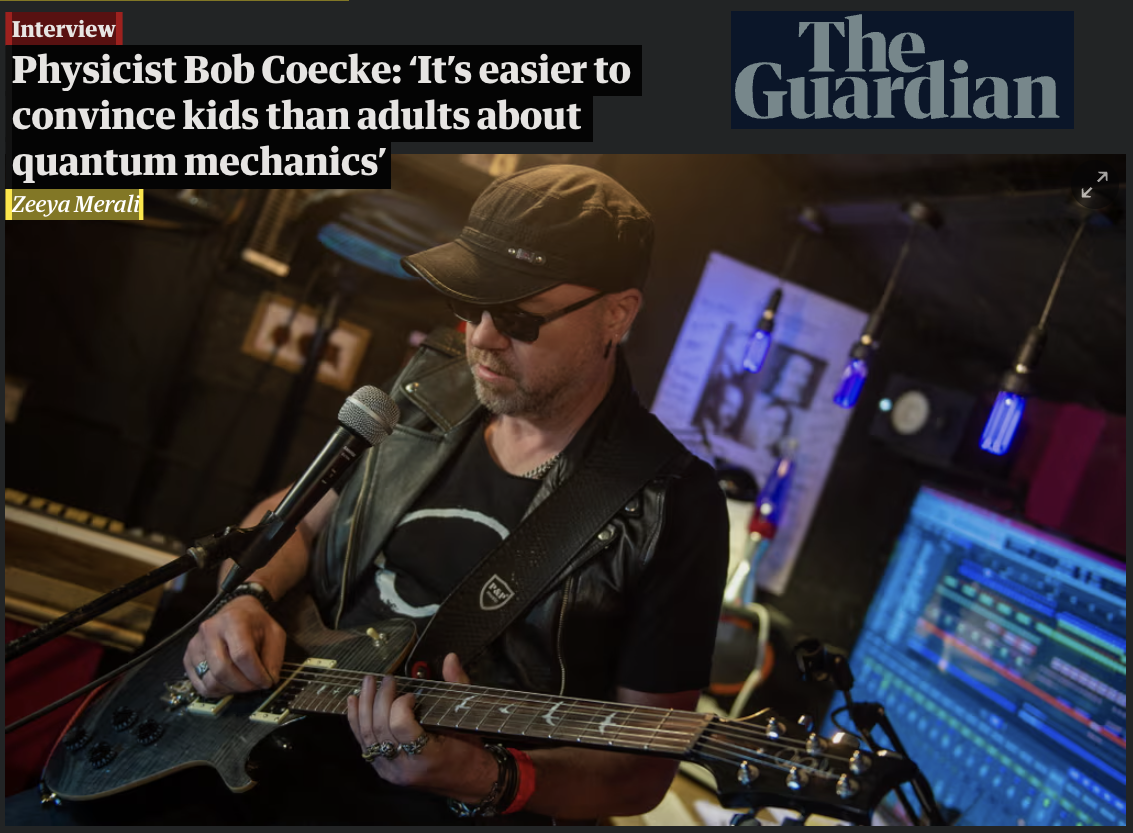
\includegraphics[width=7cm]{graphics/coecke}	
%
%Bob Coecke ~~~~\&~~~~~~Ross Duncan~\cite{cd2011}
%
%
%\onslide<2->{
%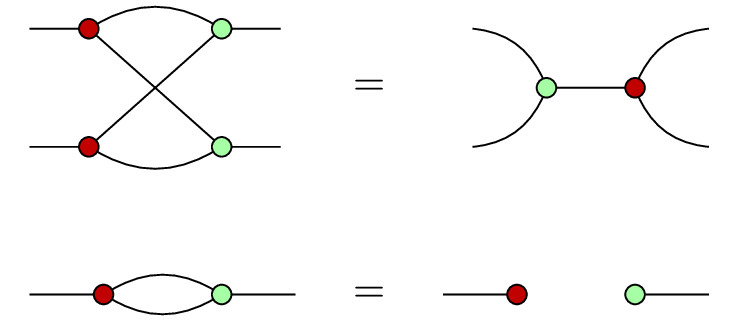
\includegraphics[width=4cm]{graphics/zx1}	
%}
%%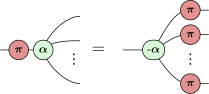
\includegraphics[width=3cm]{graphics/zx2}	
%
%
%\end{refframe}
%
%
%
%\begin{refframe}{ZX Calculus Heuristics}
%
%\begin{block}{Algorithms based on ZX calculus}
%Loop until convergence:
%\begin{enumerate}
%	\item Simplification step
%	\item Brute-force step
%\end{enumerate}
%\end{block}
%
%
%\begin{block}{Applications}
%\begin{itemize}
%	\item Simulation
%	\item Equivalence checking
%	\item Synthesis
%	\item Optimization
%\end{itemize}
%\end{block}
%
%\phantom{
%\cite{Duncan20,PyZXLS}
%}
%	
%\end{refframe}
%
%
%








